% =================================快捷键及注意事项================================
%1. 注释
%"Ctrl" + "T"
%2. 去除注释
%“Ctrl” + "U"
%*************************** 用github 提交时,只提交你修改的相关文件。日志等不提交。
\documentclass{mcmthesis}
% =================================原始控制页模板设置=======================================
\mcmsetup{CTeX = true,   % 使用 CTeX 套装时,设置为 true
        tcn = 89760, problem = B,
        sheet = false, titleinsheet = true, keywordsinsheet = true,
        titlepage = false, abstract = true}
\usepackage{palatino}
\usepackage{caption} % 图片
\usepackage{subfigure} % 图片
\usepackage{lipsum} % 文本
\usepackage{booktabs} % 表格
\usepackage{makecell} % 表格线段的粗细
\usepackage{supertabular} % 多页表格
\usepackage{float} % 去除图片浮动
\usepackage[numbers,sort&compress]{natbib} % 引入多个参考文献
\setlength{\parskip}{0.2em} %设置行距
\usepackage{indentfirst}
\usepackage{slashbox}
\newcommand{\upcite}[1]{\textsuperscript{\textsuperscript{\cite{#1}}}} % 引用上标
\setlength{\parindent}{2em}
\bibliographystyle{plain}
% =================================自制控制页设置=======================================
\newcommand{\newteamnumber}{89760} 
\newcommand{\newproblemchosen}{B} 
\newcommand{\ourtitle}{Camping on the Grand River} 
% =================================自制控制页设置=======================================
\title{Camping on the Grand River} % 标题
\author{\small \href{http://www.latexstudio.net/}
  {\graphics[width=7cm]{mcmthesis-logo}}}
\date{\today}

\begin{document}
% =================================正文设置=======================================

\begin{abstract}
\noindent	
With the rise of rafting and the growing economic benefits it generates,it is very necessary to make reasonable arrangements for the travel itinerary.
\par In this paper, we propose a two-objective optimization model.To allow the river to accommodate as many tours as possible, we set the first optimization goal, which is to maximize the number of trips per year. Secondly, we clarify the specific meaning of the contact of tour groups, followed by the construction of the second optimization goal, that is, to minimize the number of tour groups contacts. We then define the unit camping matrix, the camping matrix and the total camping matrix.Next,we take the use of camping sites for each tour, the use of arbitrary camping sites throughout the drift season, the use of all camping sites at any one night, and the number difference for two consecutive nights of camping in any group of tourists as the constraints. Considering the complexity of the solution, we weaken the second optimization goal into a constraint condition, and it can relax or tighten the constraints to adjust the scheme according to the concrete effect of the scheme implementation.
\par At the end of this article, we use $JAVA$ as a programming tool to find X = 918 for Y = 38, which means 918 trips can be made throughout the rafting season when there are 38 campsites.Then, the schedule of each plan is presented in the appendix.Finally, we analyze the sensitivity of the model. By changing the maximum drifting time per day to 7$h$,7.5$h$,8.5$h$,9$h$ ,we find that the change in the carrying capacity of the river is $ \pm 9{\rm{\% }}$ , which shows our model has better sensitivity. And by increasing the number of camps, we find that the carrying capacity of the river is generally increased by exponential.In addition, we  find that with the increase of the number of camping sites the optimal model produced when the number of contacts between groups increases correspondingly,on the actual situation.on the actual situation.on the actual situation.on the actual situation.on the actual situation.on the actual situation.on the actual situation.
\begin{keywords}
 bi-objective; optimization;0-1 matrix ; Poisson distribution
\end{keywords}
\end{abstract} % 模板自带的摘要
%\newgeometry{left=2.5cm,right=2.5cm}
 %==========================================以上不要动=================================================
  \pagestyle{empty}%
  \null%
  \vspace*{-6pc}%
  \begin{center}
  \begingroup
  \setlength{\parindent}{0pt}
     \begin{minipage}{0.28\linewidth}
      For office use only\\[4pt]
      \makebox[0.15\linewidth][l]{T1}\rule[-2pt]{0.85\linewidth}{0.5pt}\\[4pt]
      \makebox[0.15\linewidth][l]{T2}\rule[-2pt]{0.85\linewidth}{0.5pt}\\[4pt]
      \makebox[0.15\linewidth][l]{T3}\rule[-2pt]{0.85\linewidth}{0.5pt}\\[4pt]
      \makebox[0.15\linewidth][l]{T4}\rule[-2pt]{0.85\linewidth}{0.5pt}
     \end{minipage}%
     \begin{minipage}{0.44\linewidth}
      \centering
      Team Control Number\\[0.7pc]
      {\LARGE\textbf{\newteamnumber}}\\[1.8pc]
      Problem Chosen\\[0.7pc]
      {\Huge\textbf{\newproblemchosen}}
     \end{minipage}%
     \begin{minipage}{0.28\linewidth}
      For office use only\\[4pt]
      \makebox[0.15\linewidth][l]{F1}\rule[-2pt]{0.85\linewidth}{0.5pt}\\[4pt]
      \makebox[0.15\linewidth][l]{F2}\rule[-2pt]{0.85\linewidth}{0.5pt}\\[4pt]
      \makebox[0.15\linewidth][l]{F3}\rule[-2pt]{0.85\linewidth}{0.5pt}\\[4pt]
      \makebox[0.15\linewidth][l]{F4}\rule[-2pt]{0.85\linewidth}{0.5pt}
     \end{minipage}\par
     \vskip 10pt
  \rule{\linewidth}{0.5pt}\par
  \vskip 10pt
  \textbf{{\Large\the\year}\\%
%  Mathematical Contest in Modeling (MCM/ICM) Summary Sheet}%
  MCM/ICM \\
  Summary Sheet}%
  \par
  \endgroup
  \vskip 10pt
  \normalfont \Large \ourtitle \par
  \centering {\normalsize{\textbf{summary}}}
  \end{center}\par
%==========================================以上不要动=================================================







% ============================================摘要======================================================
\noindent	
With the rise of rafting and the growing economic benefits it generates,it is very necessary to make reasonable arrangements for the travel itinerary.
\par In this paper, we propose a two-objective optimization model.To allow the river to accommodate as many tours as possible, we set the first optimization goal, which is to maximize the number of trips per year. Secondly, we clarify the specific meaning of the contact of tour groups, followed by the construction of the second optimization goal, that is, to minimize the number of tour groups contacts. We then define the unit camping matrix, the camping matrix and the total camping matrix.Next,we take the use of camping sites for each tour, the use of arbitrary camping sites throughout the drift season, the use of all camping sites at any one night, and the number difference for two consecutive nights of camping in any group of tourists as the constraints. Considering the complexity of the solution, we weaken the second optimization goal into a constraint condition, and it can relax or tighten the constraints to adjust the scheme according to the concrete effect of the scheme implementation.
\par At the end of this article, we use $JAVA$ as a programming tool to find X = 918 for Y = 38, which means 918 trips can be made throughout the rafting season when there are 38 campsites.Then, the schedule of each plan is presented in the appendix.Finally, we analyze the sensitivity of the model. By changing the maximum drifting time per day to 7$h$,7.5$h$,8.5$h$,9$h$ ,we find that the change in the carrying capacity of the river is $ \pm 9{\rm{\% }}$ , which shows our model has better sensitivity. And by increasing the number of camps, we find that the carrying capacity of the river is generally increased by exponential.In addition, we  find that with the increase of the number of camping sites the optimal model produced when the number of contacts between groups increases correspondingly, which indicates that the maximum utilization of the camp and the minimum number of contacts are the optimization objectives of a pair of contradictions. Unfortunately, we do not have enough time,otherwise we will quantify the relationship between the maximum number of trips and the number of contacts with the travel team so as to find a balance point between the two based on the actual situation.
% ============================================摘要======================================================
\\
% ============================================关键字======================================================
\par
\noindent
\textbf{Key words:} bi-objective; optimization; 0-1 matrix ; Poisson distribution









 % 控制页及摘要 
\restoregeometry % 恢复原来的设置
\maketitle  % 模板自带:添加
\tableofcontents % 添加目录
\newpage % 段页
% =================================子文件夹设置====================================
% 在子文件夹下编写文件
\section{Introduction}
udhiisbsbchbas
\subsection{Background}
\noindent
There are currently about 6909 languages in the world, and the total number and geographical distribution of each language is a necessary consideration for international organizations and economic development. The so-called language population refers to the native language of the population \upcite{wiki}. In the analysis of the number of native speakers of the world language, nearly half of the population is native speakers in the following 10 languages: Mandarin (incl. Standard Chinese), Spanish, English, Hindi, Arabic, Bengali, Portuguese, Russian, Punjabi, and Japanese.

However, many people use this as their second language. The total number is not determined solely by the number of native speakers,that can determine the total number of 0.4~0.8. For a language as a second language or a third language or even more, the number of people in order and the order of the mother tongue is not the same arrangement. Therefore, when analyzing the trend of global language use, we should not only consider the number of native speakers, but also the change of the number of  second and third languages as non-native speakers. 

Over time, the increase or decrease in the total number of uses of a language is influenced by a number of factors. These factors are broadly divided into policy factors: the official language of a government or the promotion of a language, educational factors: the language of school teaching, social factors: employment pressure, cultural factors: cultural diffusion and assimilation phenomenon, demographic factors: the country's demographic changes and migration led to population migration. At the same time, due to the rapid development of the global economy, the increase of international business and transnational corporations, economic factors can drive the influence of a country's language and thus the total number of people who use language.Now the internet is popular, the world is closely related, the use of communication media and the help of mobile software, such as accurate and rapid language translation and other network factors can also affect the development of language. These factors may have an impact on the trend of language development, but not just that. 
\subsection{Restatement of the problem}
\noindent
We are required to investigate trends of global languages,and provide a multinational service company with a new international office location plan.

We understand the problem as follows:

	\begin{itemize}
		\item
We are asked to set up a model to describe the distribution of language over time based on possible influencing factors.
		\item
We should predict how the number of native speakers and total speakers will change in the next 50 years and whether the top 10 native speakers and total speakers will be replaced by another language.
		 \item
Based on the world population growth and immigration patterns for the next 50 years, we need to determine whether the geographical distribution of the language will change during this period. If so, describe the change.
		 \item 
Provide international service companies with site selection plans for new offices and consider whether the programs will be different from the perspective of long-term and short-term.
		\item 
Given the changing nature of global communications, in order to reduce the number of new international offices, we are supposed to consider additional information and give further advice based on additional information.Finally, we were also asked to write a memorandum to the relevant department. 		 	 
	\end{itemize}



\subsection{Our works} % 介绍
\section{Analysis of Overall and Key Points} % 模型的分析
\section{Assumptions and Justification}

\begin{itemize} 
	
    \item \textbf{Each month is 30 days in Drifting season, that is, the total number of days people can drifting is 180.}To simplify our model we assume 30 days per month, and this assumption is reasonable.
    
    \item \textbf{The tourists' choice of travel time complies with the Poisson distribution.}Since the choice of tourists for travel dates is unknown, the Poisson distribution is a good way to model this process and to facilitate our model building.
    
    \item \textbf{The demand for drifting is always greater than the supply.}which is a assumption based on the facts set by the context of the incident.
    
    \item \textbf{All travel teams are drifting during the day and their maximum daily drifting time is 8 hours.}According to Reference 1, we assume that the maximum daily drifting time for a tour group is 8 and the tour group can only go downstream.
    
    \item \textbf{The daily travel distance and rafting times chosen by the tour group for the same number of travel days are up to themselves.}This assumption is very realistic, river management companies will not be fixed tourist travel itinerary.
    
	\item \textbf{Assuming that for any tour group, once they have chosen the mode of transport, they will not change their means of transport for the entire journey. }We assume that the river management department to take into account the efficient use of the efficiency of the vessel, for any tour only to provide a means of transport.
	
	\item \textbf{The total number of camping sites unchanged.}According to Reference 1, we assume that there are 38 camps evenly distributed along the bank.
	
	%\begin{itemize} 
		%\item A nested item. 
		%\item[+] A ‘plus’ item. 
		%\item Another item. 
	%\end{itemize} 
	\item The total number of campsites remains unchanged, reference 1, and we assume that there are 38 camps evenly distributed along the bank. 
\end{itemize}

  % 假设
\section{Symbols and Definitions }
In the section, we use some symbols for constructing the model as follows: 
\begin{table}[htbp]
	\centering
	\caption{\label{tab:Symbols}Symbols and Definitions}
	\scalebox{0.93}[1]{%
	\begin{tabular}{c c r}
		\Xhline{1.2pt}
		Symbol  & Definition \\
		\midrule
		X &  Trips travel down the Big Long River each year during a six month period \\
		Y &  Camp sites on the Big Long River \\
		S &  The total length of the river \\
		${v_1}$ &  The speed of oarpowered rubber rafts \\
		${v_2}$ &  The speed of motorized boats \\
		${p_i}$ &  Travel options \\
		$U_i^k$ &  Unit camp matrix \\
		${C_i}$ &  Camping matrix \\
		$A$ &  Total camp camp matrix \\
		J &  The launch date of a given tour group \\
		${n_i}$ &  The number of days the  th travel option lasts \\
		$\lambda $ &  the ith dam in a series of small dams \\
		\Xhline{1.2pt}
	\end{tabular}
}
\end{table} %符号设置

\section{Models}
Multiple references are introduced.:\cite{1,2,3}

\begin{figure}[htbp]
	\centering        %居中
	\subfigure[name of the subfigure]{      %第一张子图
		\begin{minipage}{7cm}
			\centering                   %子图居中
			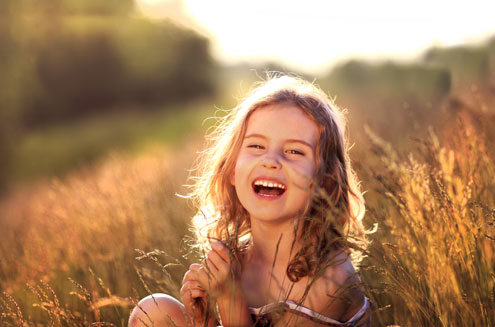
\includegraphics[scale=0.4]{one_3.jpg}          %以pic.jpg的0.5倍大小输出
		\end{minipage}}
	\subfigure[name of the subfigure]{          %第二张子图
		\begin{minipage}{7cm}
			\centering                                                          %子图居中
			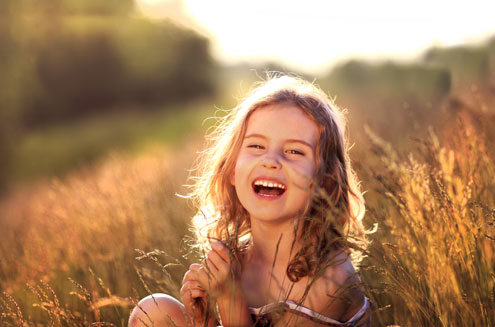
\includegraphics[scale=0.4]{one_3.jpg}         %以pic.jpg的0.5倍大小输出
		\end{minipage}}
	\caption{the figure} %          %大图名称
	\label{fig:123}      %图片引用标记
\end{figure}

Refer to the test for Figure \ref{fig:123}


\begin{figure}[h]
	\small
	\centering
	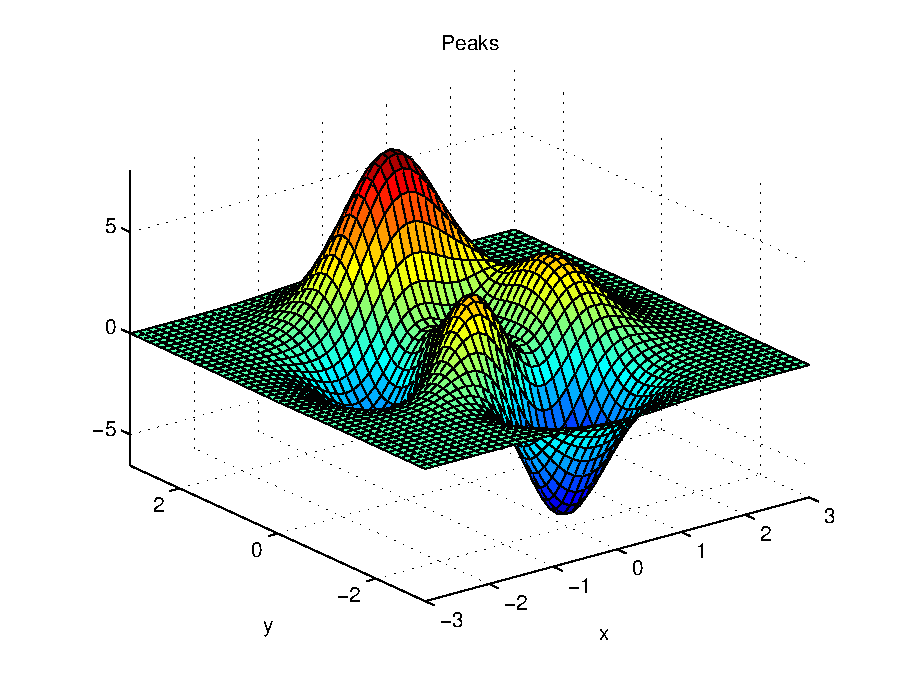
\includegraphics[width=12cm]{mcmthesis-aaa.eps}
	\caption{aa} \label{fig:aa}
\end{figure}





\begin{equation}
a^2 \label{aa1}
\end{equation}
about this eqref \eqref{aa1}

 % 模型
\section{Conclusions} % 结论
\section{Sensitivity analysis of the model}
\noindent
Since a good mathematical model should have good sensitivity, we conduct a sensitivity analysis of the model we built. In this section, we will conduct a sensitivity analysis of the maximum daily drifting time, the number of campsites evenly distributed along the banks, the minimum number of collisions during the drifting season.
\subsection{Sensitivity analysis of the maximum drifting time of a day}
\noindent
In the hypothetical part, we assume that the maximum daily drifting time for a tour group is 8h, whereas the different maximum daily drifting durations will change the maximum number of trips. We have substituted the maximum daily drifting durations 7h, 7.5h, 8.5h, and 9h into our model The results are as follows:	
\begin{table}[htbp]
	\centering
	\caption{\label{tab:Symbols}The results}
	\begin{tabular}{c|c c c c r}
		\Xhline{1.2pt}
		Daily maximum drifting time/h  & 7.0  & 7.5 & 8.0 & 8.5 & 9.0 \\
		\midrule
		Raiver carrying capacity/times & 842 & 874 & 918 & 931 & 948 \\
		\Xhline{1.2pt} 
	\end{tabular}
\end{table}
The rate of change of the carrying capacity of the river by the table:
\begin{equation}
\begin{array}{l}
{\Delta _1}{\rm{ = }}\frac{{842 - 918}}{{918}} \times 100{\rm{\%  =  - }}8.2{\rm{\% }}\\
\\
{\Delta _2}{\rm{ = }}\frac{{948{\rm{ - }}918}}{{918}} \times 100{\rm{\%  = }}3.2{\rm{\% }}
\end{array}\label{aa1}
\end{equation}
\par According to the result of sensitivity test, we find that the variation range of river carrying capacity does not exceed, proving that our model has better sensitivity.

\subsection{Sensitivity analysis of the total campsite}
\noindent
Obviously, the carrying capacity of a river is positively related to the number of campsites. In order to study the relationship between the increasing trend of the maximum number of trips X during the drift season and the total number of campsites Y in our model, we ensure that the number of fleet contacts will not change , Change the number of campsites and observe the growth trend of the maximum number of trips, and then use function fitting to roughly determine the change of the maximum number of trips with the total campsite growth. Suppose the total number of campgrounds is 26, 30, 34, 38, 42, 46, 50 and enter the model to get the result as follows:\\

\begin{table}[htbp]
	\centering
	\caption{\label{tab:Symbols}The results}
	\scalebox{0.89}[0.85]{%
	\begin{tabular}{cccccccc}
		\Xhline{1.2pt}
		Number of camps & 26 & 30 & 34 & 38 & 42 & 46 & 50 \\
		\midrule
		Raiver carrying capacity/times & 805 & 880 & 892 & 918 & 927 & 932 & 934 \\
		\midrule
		The rate & -8.54\% & -4.21\% & -2.78\% & 0\% & 1.06\% & 0.52\% & 0.21\% \\ 
		\Xhline{1.2pt} 
	\end{tabular}%
	}
\end{table}

\par Where, the growth rate\\
\begin{equation}
\Delta {\rm{ = }}\left\{ {\begin{array}{*{20}{c}}
	{\frac{{{Y_n} - {Y_{n + 1}}}}{{{Y_{n + 1}}}}}&{n < 38}\\
	\\
	{\frac{{{Y_{n + 1}} - {Y_n}}}{{{Y_n}}}}&{n > 38}
	\end{array}} \right.\label{aa1}
\end{equation}
\par It is easy to find through analysis of R that X and Y are roughly in exponential relation with the increase of the total number of camping sites evenly distributed along the bank, the maximum number of trips in the drifting season will increase less and less and eventually may show a saturated trend.

\subsection{Sensitivity analysis of contacts frequency}
\noindent
In the process of solving the model, we weaken the second optimal objective( the number of contect) into the constraint condition, next we change the minimum contact number M to ensure the total number of the camp, and observe the change of the maximum travel times of the drift season, that is, the river carrying capacity X. We will take M in the sequence of 8,10,12,14,16, and the result is as follows:
\begin{table}[htbp]
	\centering
	\caption{\label{tab:Symbols}the sequence of 8,10,12,14,16, and the results}
	\scalebox{0.89}{%
		\begin{tabular}{c|ccccc}
			\Xhline{1.2pt}
			Number of contacts  & 8 & 10 & 12 & 14 & 16 \\
			\midrule
			river carrying capacity / Times & 907 & 918 & 928 & 937 & 942 \\
			\Xhline{1.2pt} 
		\end{tabular}%
	}
\end{table}
\par Our analysis of the above table shows that the maximum number of trips increases when the number of contacts with the group is allowed to increase. Taking into account the number of campsites and the number of contacts on the maximum number of trips, it is not difficult to find that the two optimization objectives in this model are contradictory. Therefore, we should conduct an in-depth study on the relationship between the two. Unfortunately, due to time constraints, we failed to accomplish the task. If there is a chance later, we must make up for this great regret % 灵敏度分析
\section{Strengths and weaknesses}
\subsection{Strengths}
\begin{itemize}
	\item \textbf{Improve the existing model}
	\par Existing indicators of linguistic influence assessment model change and the evaluation of linguistic effectiveness that is more suitable for solving this problem are improved. To quantify the linguistic influence of the abstract description to a fraction of [0,1] and calculate the language score to provide a reasonable basis for the new international office location
	\item \textbf{Good flexibility}
	\par To study this problem, two main models are established: the non-equidistant GM (1,1) prediction model and the language performance evaluation model (LII)
	\par The former model can be used for other forecasting problems. The latter model can be extended to the evaluation problem. The model is more flexible and can be transformed into a solution to other practical problems
	\item \textbf{youdian}
	
	\item \textbf{youdian}
	
\end{itemize}

\subsection{weaknesses}

\begin{itemize}
	\item \textbf{Inaccuracy}
	\item \textbf{Simplifying assumptions}
	\item \textbf{Lack of data}
\end{itemize}
\section{Future Improvements} %进一步提高
\input{paper/Memorandum} % 说明书
% =================================================================

\begin{thebibliography}{99}
	\addcontentsline{toc}{section}{References} % 在目录中添加参考文献
		
	\bibitem{1}\url{http://canyonx.com/trip_lengths_logistics.php}
	\bibitem{2}Shang Pengchao, Zhang Cong, Ren Qingfeng, et al.Arrangement of drifting travel plan [J] .Journal of Yan'an University (Natural Science Edition), 2012, 31 (3): 48-50.
	Addison-Wesley Publishing Company, 1986.
	\bibitem{3}XU Dao, CAO Xiaoyu, GENG Jianghua.Application of 0-1 Integer Programming Model to Rafting Travel Schedule [J]. Science Technology Information, 2012 (27): 158-158.
\end{thebibliography}


\begin{appendices}

\section{First appendix}

\lipsum[13]

Here are simulation programmes we used in our model as follow.\\

\textbf{\textcolor[rgb]{0.98,0.00,0.00}{Input matlab source:}}
\lstinputlisting[language=Matlab]{./code/mcmthesis-matlab1.m}

\section{Second appendix}

some more text \textcolor[rgb]{0.98,0.00,0.00}{\textbf{Input C++ source:}}
\lstinputlisting[language=C++]{./code/mcmthesis-sudoku.cpp}

\end{appendices} 
% =================================子文件夹设置====================================
\end{document}
